
\section{Intersections, intention and scenarios}
\label{sec:intro_intersections}
When it comes to the scenarios considered in this work. This section aims to clarify the use of the words' intersection, intention and scenario.
% When a pedestrian approach a crossing they have been taught at a young age to look at both sides of the road before crossing. The same apply for a human driver approaching an intersection. 
% When a human driver approach an intersection, it is natural to observe the environment to identify the traffic light, signs and other approaching vehicles. Then assess the situation, who has the right of way? 

% The intention of the other driver can be guided by the 
% Recently nontraditional intersections are also becoming increasingly popular. The goal of these designs is to reduce the number and/or severity of conflict points by altering the customary vehicular paths at the intersection. In light of the increased focus on and occurrence of these intersection types, it is expected that the application of nontraditional designs will continue to spread.

\begin{figure}[h]
	\centering
	\begin{subfigure}[t]{0.48\columnwidth}
		\centering
		\begin{tikzpicture}
			% Crossing
			\def\crossleftx{-2}
			\def\crossrightx{2}
			\def\crosstopy{2}
			\def\crossboty{-2}
			\def\roadwidth{0.5}

			\draw (0,0) circle (2pt);
			\node at (1.2, 0.2) {conflict point};
			\draw[thick] (\crossleftx, \roadwidth) -- (-\roadwidth, \roadwidth) -- (-\roadwidth, \crosstopy);
			\draw[thick] (\crossleftx, -\roadwidth) -- (-\roadwidth, -\roadwidth) -- (-\roadwidth-\roadwidth, \crossboty);
			\draw[thick] (\roadwidth, \crosstopy) -- (\roadwidth, \roadwidth) -- (\crossrightx, \roadwidth);
			\draw[thick] (\roadwidth-\roadwidth, \crossboty) -- (\roadwidth, -\roadwidth) -- (\crossrightx, -\roadwidth);

			% 	cars
			\node[inner sep=0pt] (ego_car) at (\crossleftx+0.5,0)
			{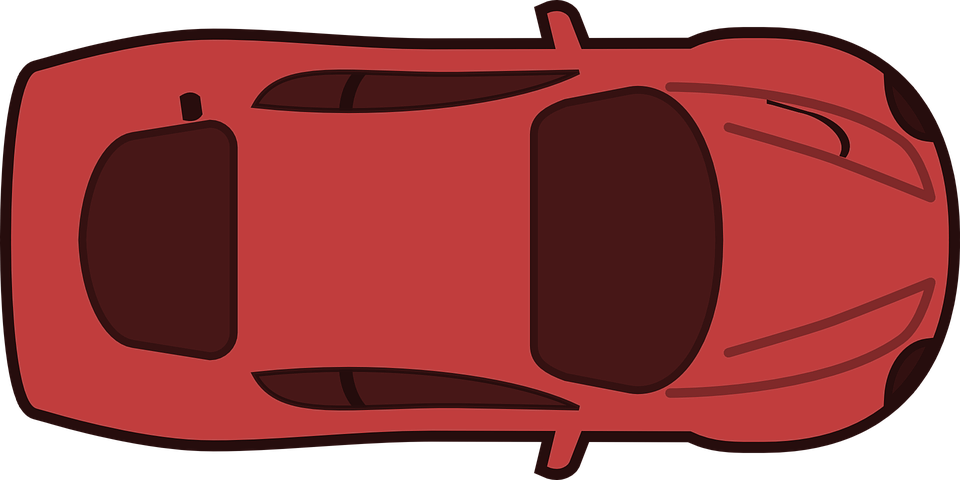
\includegraphics[width=.18\textwidth, angle=0]{figures/ego_car_top_down.png}};

			\node[inner sep=0pt] (target_car) at (0,\crosstopy-0.5)
			{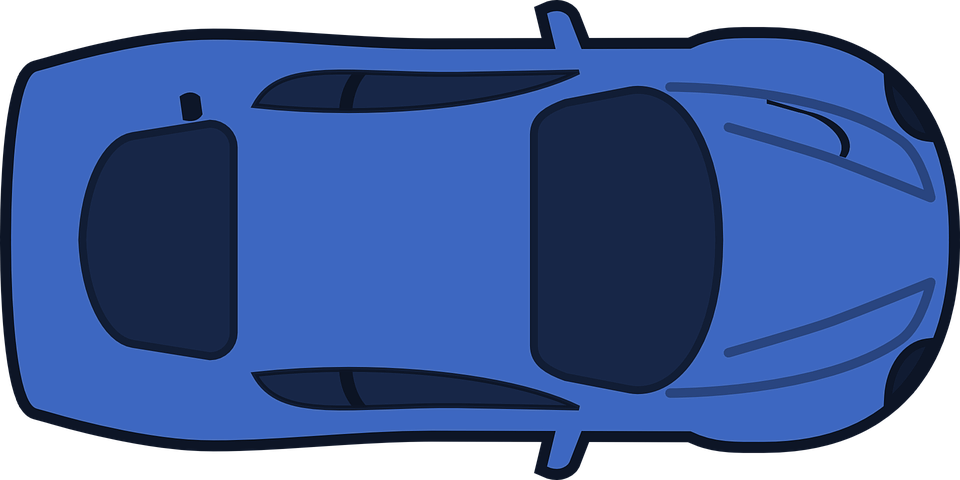
\includegraphics[width=.18\textwidth, angle=-90]{figures/target_car_top_down.png}};

			\node[inner sep=0pt] (target_car) at (-.1,-0.8)
			{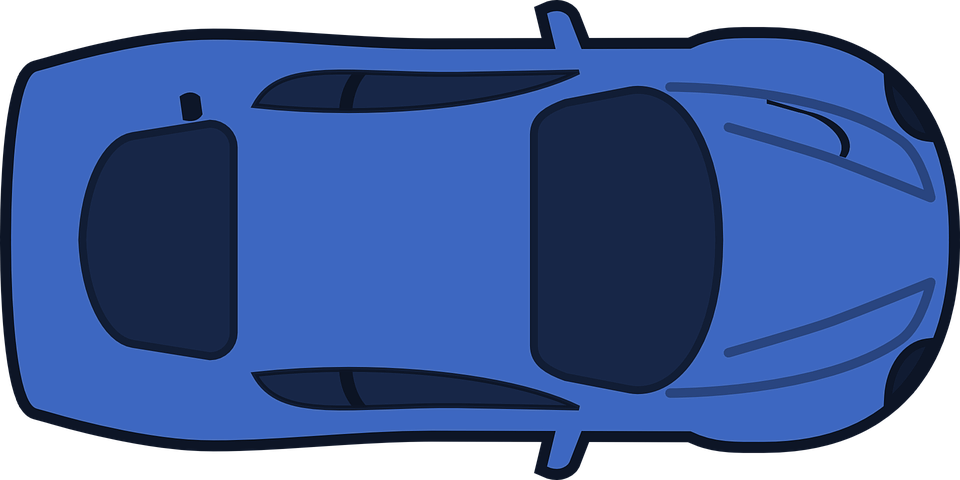
\includegraphics[width=.18\textwidth, angle=-110]{figures/target_car_top_down.png}};


		\end{tikzpicture}
		\caption{Single intersection}
\end{subfigure}%
	~ 
	\begin{subfigure}[t]{0.48\columnwidth}
		\centering
		\begin{tikzpicture}
			% Crossing
			\def\crossleftx{-2.5}
			\def\crossrightx{2.5}
			\def\crosstopy{2}
			\def\crossboty{-2}
			\def\roadwidth{0.5}

			\draw (-0.5,0) circle (2pt);
			\draw (0.5,0) circle (2pt);
			% \node at (0.7, 0.2) {crossing point$^1$};
			\draw[thick] (\crossleftx, \roadwidth) -- (-\roadwidth-0.5, \roadwidth) -- (-\roadwidth-0.5, \crosstopy);
			\draw[thick] (\crossleftx, -\roadwidth) -- (-\roadwidth-0.5, -\roadwidth) -- (-\roadwidth-0.5, \crossboty);
			\draw[thick] (0, \crosstopy) -- (0, \roadwidth);
			\draw[thick] (0, -\roadwidth) -- (0, \crossboty);
			\draw[thick] (\roadwidth+0.5, \crosstopy) -- (\roadwidth+0.5, \roadwidth) -- (\crossrightx, \roadwidth);
			\draw[thick] (\roadwidth+0.5, \crossboty) -- (\roadwidth+0.5, -\roadwidth) -- (\crossrightx, -\roadwidth);

			% 	cars
			\node[inner sep=0pt] (ego_car) at (\crossleftx+0.5,0)
			{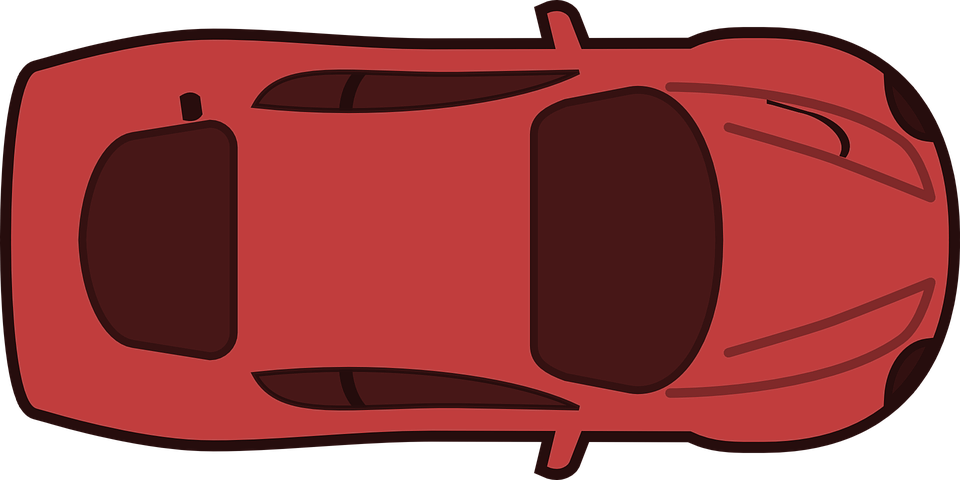
\includegraphics[width=.18\textwidth, angle=0]{figures/ego_car_top_down.png}};

			\node[inner sep=0pt] (target_car) at (-0.5,\crosstopy-0.5) {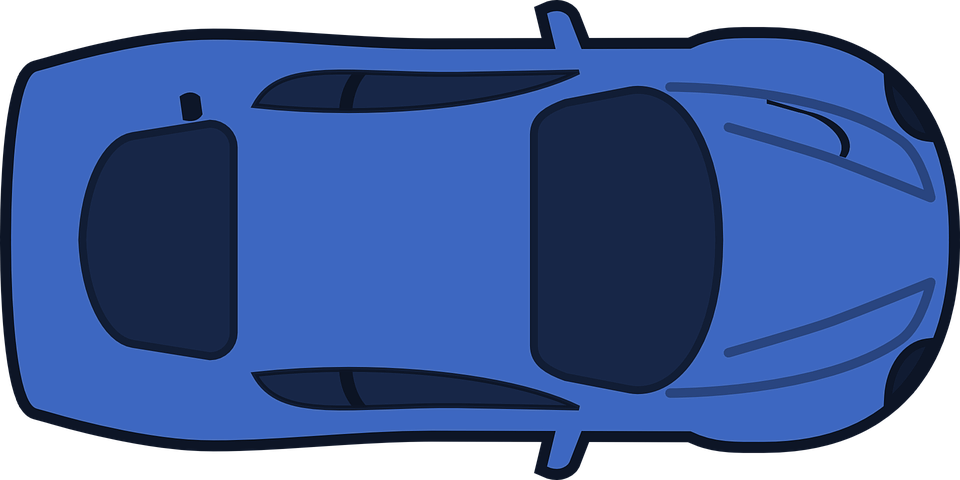
\includegraphics[width=.18\textwidth, angle=-90]{figures/target_car_top_down.png}};

			\node[inner sep=0pt] (target_car_2) at (0.5,\crossboty+0.5) {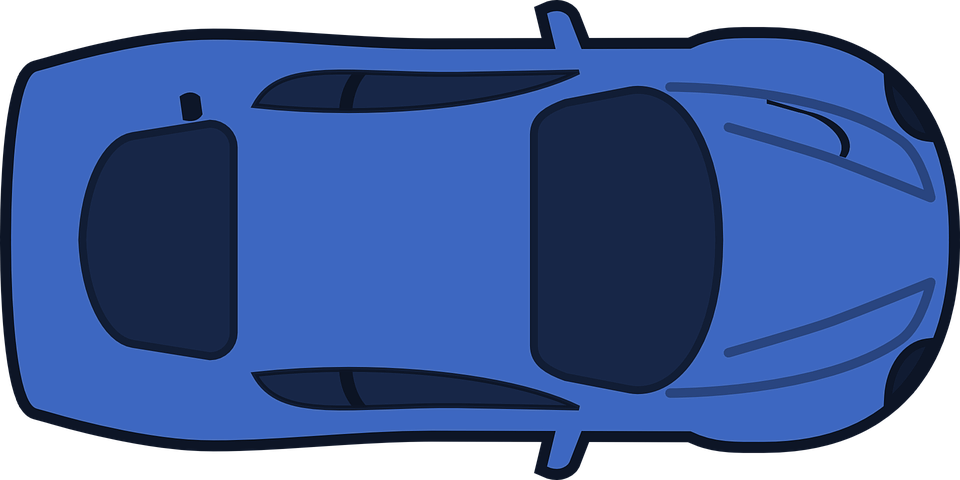
\includegraphics[width=.18\textwidth, angle=90]{figures/target_car_top_down.png}};

		\end{tikzpicture}
		\caption{Double intersection}
	\end{subfigure}

	\caption{Examples of different intersections}
	\label{fig:example_intersections}

\end{figure}
An intersection refers the geometrical shape of the roads intersecting each other e.g., number of junctions, conflict points, turns and angle of incidence, as shown in Figure~\ref{fig:example_intersections}. 
An intersection can either be signalized or unsignalized, a signalized intersection has something to define the right-of-way e.g., a regulatory (i.e., STOP or YIELD) sign or a traffic signal, while an unsignalized intersection does not. But as mentioned in the introduction, humans do not always follow these right-of-way rules and therefore end up in accidents. That is why this thesis defines the intentions as what other vehicle will do in the future: stop, slow down or drive through the intersection. If the intention is known, then all intersections can be treated as unsignalized since the right-of-way can be implied by the intention instead of the infrastructure. This way, even when another vehicle would break a traffic rule and run a red light, a good agent would still stop and be safe. 
%  Intersections in the world often have something to decide the right of way like traffic rules, signs or lights. 
% While there exists a large variation of intersections in the world, this work only focus on the decision to drive or yield, we can reduce the dimention to 1. 

Finally, the combination of an intersection, its traffic participants, their intentions, positions and velocities. 
More detail on the specific intersections and scenarios considered in this work is presented in Chapter~\ref{ch:modeling_intersection}.

% \begin{figure}[h]
% 	\centering
% 	\begin{subfigure}[t]{0.48\columnwidth}
% 		\centering
% 		\begin{tikzpicture}
% 			% Crossing
% 			\def\crossleftx{-2}
% 			\def\crossrightx{2}
% 			\def\crosstopy{2}
% 			\def\crossboty{-2}
% 			\def\roadwidth{0.5}

% 			\draw (0,0) circle (2pt);
% 			% \node at (1.2, 0.2) {crossing point};
% 			\draw[thick] (\crossleftx, \roadwidth) -- (-\roadwidth, \roadwidth) -- (-\roadwidth, \crosstopy);
% 			\draw[thick] (\crossleftx, -\roadwidth) -- (-\roadwidth, -\roadwidth) -- (-\roadwidth, \crossboty);
% 			\draw[thick] (\roadwidth, \crosstopy) -- (\roadwidth, \roadwidth) -- (\crossrightx, \roadwidth);
% 			\draw[thick] (\roadwidth, \crossboty) -- (\roadwidth, -\roadwidth) -- (\crossrightx, -\roadwidth);

% 			% 	cars
% 			\node[inner sep=0pt] (ego_car) at (\crossleftx+0.5,0)
% 			{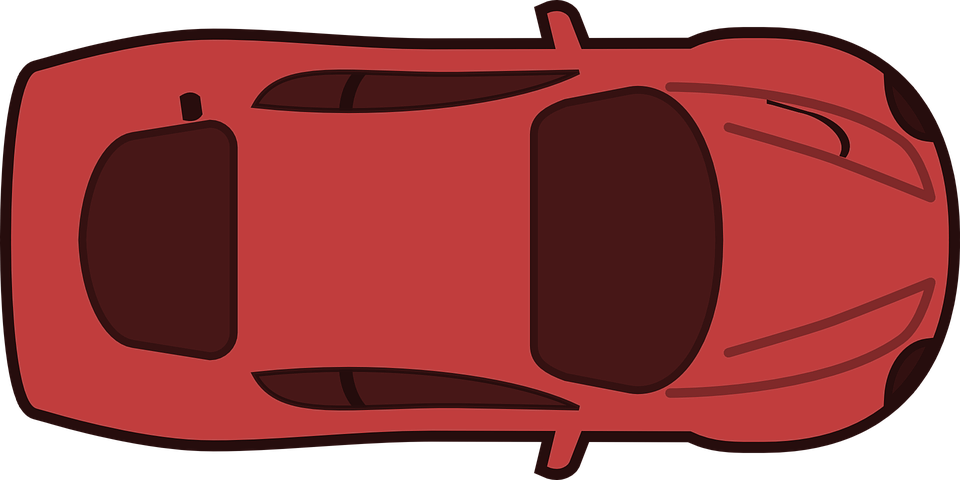
\includegraphics[width=.18\textwidth, angle=0]{figures/ego_car_top_down.png}};

% 			\node[inner sep=0pt] (target_car) at (0,\crosstopy-0.5)
% 			{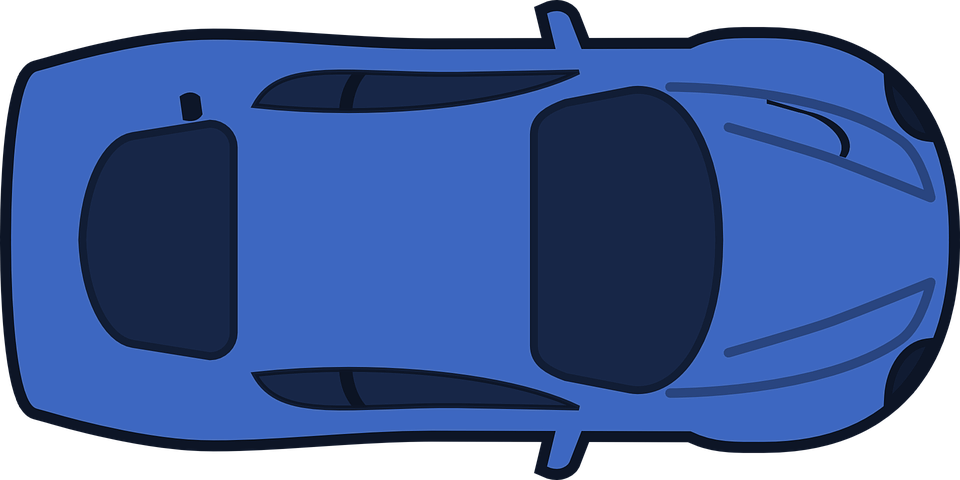
\includegraphics[width=.18\textwidth, angle=-90]{figures/target_car_top_down.png}};

% 			%  \node[inner sep=0pt] (targetcar2) at (0,2.5)
% 			%  {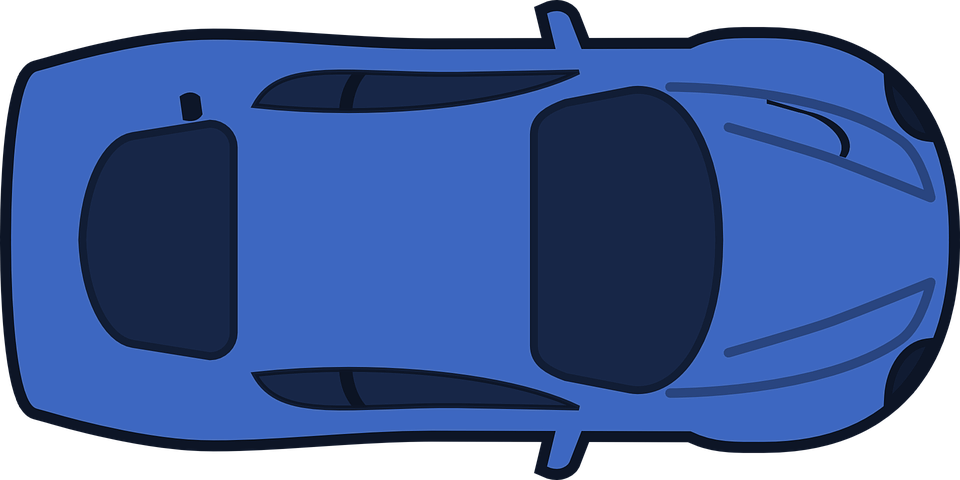
\includegraphics[width=.18\textwidth, angle=-90]{figures/target_car_top_down.png}};
% 			%  \node (tctext2) [right=of targetcar2] {Car 2};
			
% 			% \node[inner sep=0pt] (target_car_1) at (0,-1.5)
% 			% {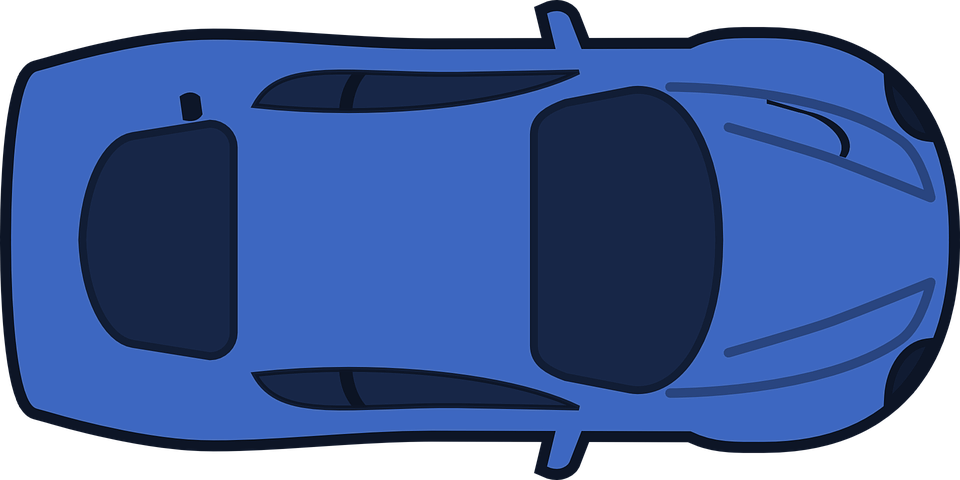
\includegraphics[width=.18\textwidth, angle=-90]{figures/target_car_top_down.png}};
% 			% \node (tc_text1) [right=of target_car_1] {Car 1};
% 		\end{tikzpicture}
% 		\caption{Single intersection scenario}
% \end{subfigure}%
% 	~ 
% 	\begin{subfigure}[t]{0.48\columnwidth}
% 		\centering
% 		\begin{tikzpicture}
% 			% Crossing
% 			\def\crossleftx{-2.5}
% 			\def\crossrightx{2.5}
% 			\def\crosstopy{2}
% 			\def\crossboty{-2}
% 			\def\roadwidth{0.5}

% 			\draw (-0.5,0) circle (2pt);
% 			\draw (0.5,0) circle (2pt);
% 			% \node at (0.7, 0.2) {crossing point$^1$};
% 			\draw[thick] (\crossleftx, \roadwidth) -- (-\roadwidth-0.5, \roadwidth) -- (-\roadwidth-0.5, \crosstopy);
% 			\draw[thick] (\crossleftx, -\roadwidth) -- (-\roadwidth-0.5, -\roadwidth) -- (-\roadwidth-0.5, \crossboty);
% 			\draw[thick] (0, \crosstopy) -- (0, \roadwidth);
% 			\draw[thick] (0, -\roadwidth) -- (0, \crossboty);
% 			\draw[thick] (\roadwidth+0.5, \crosstopy) -- (\roadwidth+0.5, \roadwidth) -- (\crossrightx, \roadwidth);
% 			\draw[thick] (\roadwidth+0.5, \crossboty) -- (\roadwidth+0.5, -\roadwidth) -- (\crossrightx, -\roadwidth);

% 			% 	cars
% 			\node[inner sep=0pt] (ego_car) at (\crossleftx+0.5,0)
% 			{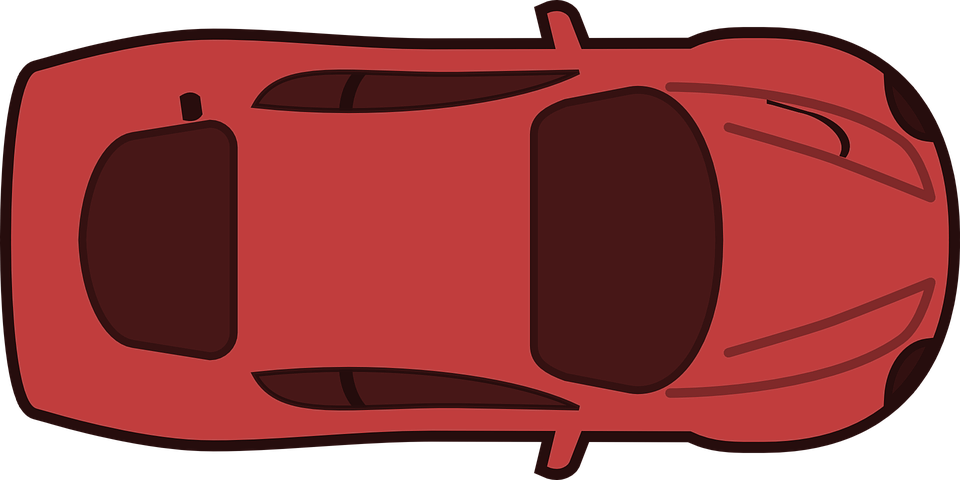
\includegraphics[width=.18\textwidth, angle=0]{figures/ego_car_top_down.png}};

% 			\node[inner sep=0pt] (target_car) at (-0.5,\crosstopy-0.5)
% 			{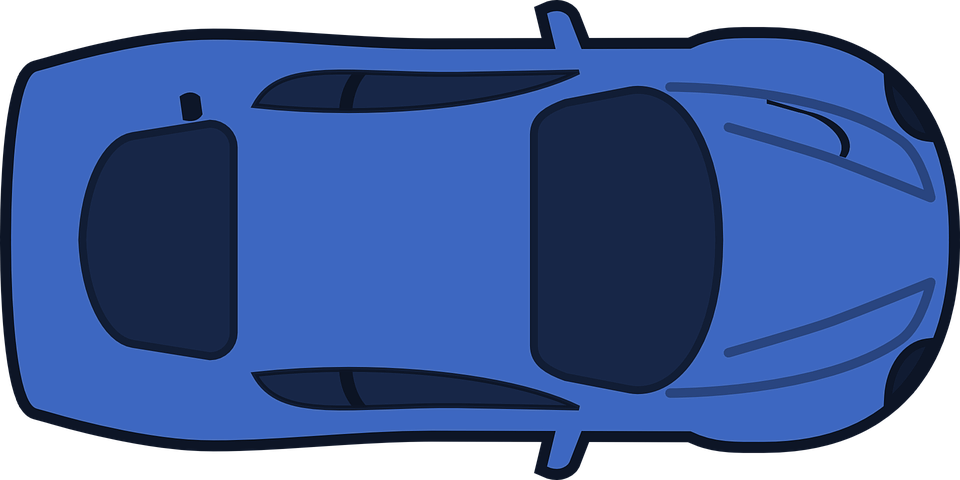
\includegraphics[width=.18\textwidth, angle=-90]{figures/target_car_top_down.png}};

% 			\node[inner sep=0pt] (target_car_2) at (0.5,\crossboty+0.5)
% 			{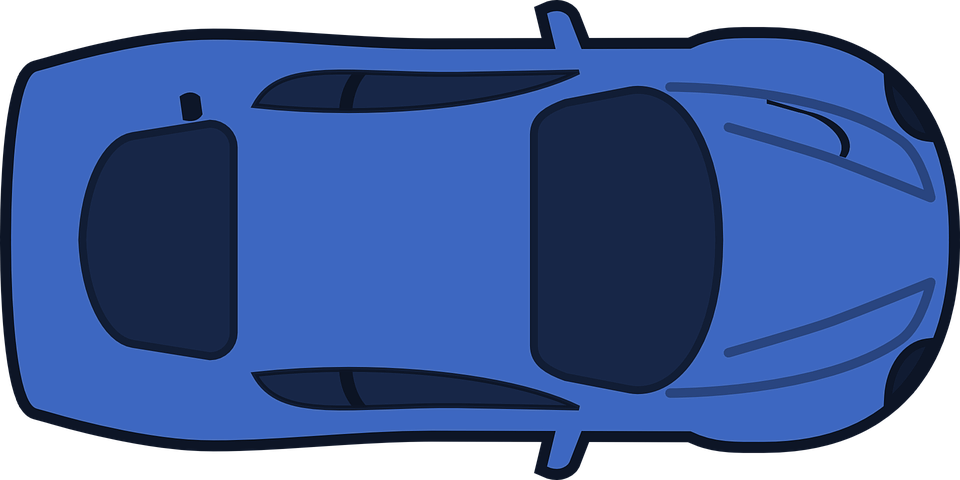
\includegraphics[width=.18\textwidth, angle=90]{figures/target_car_top_down.png}};
% 		\end{tikzpicture}
% 		\caption{Double intersection scenario}
% 	\end{subfigure}

% 	\caption{Examples of different scenarios}
% 	\label{fig:example_scenarios}

% \end{figure}

% \tommy{what I want to say here is: define an unsignalized intersection. There are many variations. Roundabouts are defined as unsignalized intersection. To satisfy the requirement of being able to drive anywhere for level 5 it is necessary to find a method that can scale to these different scenarios}

%  In light of the increased focus on and occurrence of these intersection types nationwide, it is expected that the application of nontraditional designs will continue to spread.
